\lfoot{Autor: Daniel Melichar}
\subsubsection{Relationale Datenbanken}
\label{subsec:relationaleDB}

Die relationale Datenbank ist seit dem ersten Erscheinen in 1970 weit gekommen und ist von den meisten Großkonzernen der Welt adaptiert worden. Mit der eigens dafür entwickelten \textit{Programmiersprache} SQL (Structured Query Langauge) war das umgehen mit Datenbanken und Tabellen und der darin gespeicherten Information so einfach wie noch nie.

\begin{figure}[!htb]\centering
	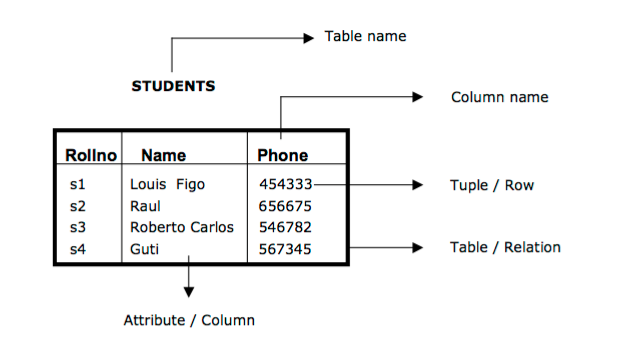
\includegraphics[width=0.5\textwidth]{images/relationaleTabelle}
	\caption{Beispiel einer relationalen Datenbank}
\end{figure}

Features von relationalen DBMS (Achtung: diese sind stark vom eigentlichem DBMS abhängig)
\begin{itemize}
\item Unterstützt eine große Menge an Daten
\item Datensicherheit durch backups, permissions, etc.
\item Fehler Toleranz und Wiederherstellung
\end{itemize}

Hinter den Kulissen sorgt das Relational Database Management System (RDBMS) dafür das die Eigenschaften des ACID (Atomicity, Consistency, Isolation, Durability) Prinzips der Transaktionen so funktionieren wie sie sollen. Beachtet man nun auch die anderen Features der Sprache, so wie Constraints (primary and foreign keys, Datentype, etc.) oder Stored Procedures/Functions, erkennt man schnell, dass je mehr Information eine relationale Datenbank enthält, desto langsamer wird sie.

Einige der größten Limitierungen \cite{MELD.CH2-relationaleDB.rdbmsBuch} durch das relationale Datenbank Model sind
\begin{itemize}
\item Skalierbarkeit: ab einem gewissen Zeitpunkt muss die Datenbank über mehrere Server laufen da ein Server nicht mehr genügend Ressourcen verfügt um die Daten zu managen
\item Komplexität: die Daten müssen zu Tabellen strukturiert werden; es ist also ein Schema notwendig
\item Features: Meist für Datenintegrität aber nicht für Datenverarbeitung 
\end{itemize}


Zusammenfassed kann man also sagen, dass die Verwendung eines RDBMS dann sinn macht, wenn man ein Datenschema erstellen kann. Das bedeutet konkret: wenn man weiß welche Daten man hat und haben wird, wie man diese in eine Tabellen Struktur einbauen kann, und man Anforderungen die sich nur im geringen Maß ändern können ist es sinnvoll ein RDBMS zu verwenden. Die zur Verfügung gestellten Features werden einen Administrator sehr gut unterstützen. 


\subsubsection{Nicht relationale Datenbanken (NoSQL)}
\label{subsec:nichtrelationaleDB}

In diesem Kapitel werden ein Einblick in das Konzept von nicht-relationalen Datenbanken gegeben. Es wird nicht über die ersten Systeme gesprochen die damals dem NoSQL-Movement angehörten (Objekt-Datenbanken, XML-Datenbanken, Datenbanken für spezielle Anwendungsgebiete wie Analyse oder Streamprozessoren) diese sollten aber zumindest erwähnt werden.

\paragraph{Motive und Beweggründe}
Der Term \textit{NoSQL} wurde erstmalig in 1998 für eine relationale Datenbank, welche ohne der SQL-Sprache funktioniert, verwendet\cite{MELD.CH2-noSQL.firstSQLNaming}. Der Term wurde dann wieder in über die Jahre von verschiedensten Leuten aufgenommen. Unglücklicherweise gab es keine definitive Beschränkung für welche Datenbanksysteme zum NoSQL-Movement gehören. Durch den Blogger und Rackspace Mitarbeiter, Eric Evans, ist der Term ganz besonders bekannt geworden – er sagte hierzu: \cite[\textit{“the whole point of seeking alternatives is that you need to solve a problem that relational databases are a bad fit for”}]{MELD.CH2-noSQL.whatsInAName}

Das bekannte IT und Technologie Magazine \textit{Computerworld} hat in 2009 bei einer NoSQL Konferenz in San Franciso die dort vorhanden Developer befragt wieso NoSQL gegenüber relationalen Datenbanken im Vorteil liegt\cite{MELD.CH2-noSQL.whyItsBetter}.

Die folgenden Erklärungen wurden von den Entwicklern gemacht.
\begin{itemize}
	\item \textbf{Unnötige Komplexität wird vermieden}\newline
	 Relationale Datenbanken verfügen über eine große Anzahl an Features und strikter Daten Konsistenz Vorschriften. Jedoch kann diese Anzahl an Features und die Anbindung an das ACID-Model zu viel für spezifische Anwendungsfälle sein. Zum Beispiel ist die Überprüfung von Session Daten die Mehrmals als Kopie abgespeichert sind nicht notwendig.

	\item \textbf{Hohe Verarbeitungsmenge}\newline
	 Manche NoSQL Datenbanken verfügen über eine weitaus größere 	Verarbeitungsmenge. So wird bei dem column-store Hypertable, welches die Ziele von Google’s BigTable verfolgt, erlaubt es bis zu einer Millionen Datensätze pro Tag zu speichern. Ein weiteres Beispiel ist Google’s BigTable selbst; es kann bis zu 20 Petabyte pro Tag verarbeiten.

	\item \textbf{Horizontale Skalierbarkeit und geringe Hardware requirements}\newline
	 Im Vergleich mit relationalen DBMS sind die meisten NoSQL Datenbanken so konzipiert um horizontale Skalierung möglichst einfach durchzuführen. Horizontale Skalierung bedeutet prinzipiell mehr Server, oder im allgemeinen Verarbeitungsmachinen, in den Pool der Ressourcen hinzu zu fügen. Es gibt zwar auch eine äquivalente Verbesserungsmöglichkeitne für RDBMS, das so genannte \textit{sharding}, dies ist oft aber weit aus komplizierter als bei NoSQL. Zum Beispiel gibt es bei der Bekannten NoSQL Datenbank \textit{MongoDB} eine automatische Version der Sklaierung.

	\item \textbf{Object-Relational Mapping wird vermieden}\newline
	 Auch hier verwenden die meisten NoSQL Datenbanken eine Struktur zur Speicherung der Daten die entweder sehr Simple oder sehr Ähnlich zu jenen sind die auch bei Objekt-Orientierten-Programmiersprachen aufzufinden sind. Hierfür ist dann kein ressourcenintensives Object-Relational Mapping notwendig.
\end{itemize}

Zu diesem Bericht gab es dann auch einen Blog post von Nati Shalom, CTO und Gründer von GigaSpaces. Er hat die folgenden weiteren Punkte für die NoSQL-Bewegung aufgestellt\cite{MELD.CH2-noSQL.natiShalomlol}.

\begin{itemize}
	\item \textbf{Komplexität und benötigter Aufwand bei Datenbank Clustern}\newline
	 Er meint, dass NoSQL Datenbanken auf eine Art und Weise entwickelt worden sind, die das erstellen von Clustern sehr einfach macht. Unter anderem spielt hier auch das bereits angesprochene Skalieren auf horizontaler Ebene eine große Rolle.
	
	\item \textbf{Kompromiss zwischen Performance und Verlässlichkeit}\newline
	 Shalom behauptet außerdem, dass verschiedene Szenarien gibt, in welchen Applikationen den Fokus auf Performance legen und nicht auf Verlässlichkeit. Ein gutes Beispiel für dieses Szenario sind die Daten von HTTP Sessions – diese müssen zwischen vielen Web Servern geschickt werden, löschen sich aber dann sobald der User sich abmeldet.

	\item \textbf{Cloud Computing}\newline
	 Hier werden sehr oft NoSQL Lösungen verwendet, da dass Limit der Skalierbarkeit sehr hoch, bis sogar unendlich ist, es wenig administrative Tätigkeiten im Umgang mit NoSQL gibt, es viele NoSQL Datenbanken gibt die spezifisch für Datawarehousing entiwckelt worden sind, uvm.
\end{itemize}

\paragraph{Techniken und Konzepte\newline}
\htab\textbf{Das CAP-Theorem\newline}
Das von Eric Brewer im Jahre 2000 entwickelte CAP-Theorem ist heutzutage in vielen Web-Unternehmen (z.B. Amazon) aber auch in der NoSQL Community aufzufinden\cite{MELD.CH2-noSQL.capTheorem}. Der CAP Akronym steht für:

\begin{itemize}
	\item \textit{Consistency:} Ob und wie ein System in den konsistenten Zustand, nach Ausführung einer Operation, zurück gelangt. Ein verteiltes System wird im Normalfall als Konsistent bezeichnet, wenn alle lesenden Teile das selbe Resultat aus dem geteilten Informationspool bekommen.

	\item \textit{Availability:} Hierbei ist vor allem auf das Design und Umsetzung eines Systems zu achten. Es sollte so entwickelt sein, dass bei Ausfall eines Servers in einem Cluster immer noch die selben Operationen durchgeführt werden können.

	\item \textit{Partition Tolerance:} Anders als bei Availability geht es hier meistens um Netzwerk Partitionen und die Möglichkeit weiter Operationen durchzuführen, wenn zwei Netzwerke im System nicht miteinander kommunizieren können.
\end{itemize}

 Brewer behauptet, dass man nur zwei von diesen drei Eigenschaften in einem \textit{shared-data system} haben kann\cite{MELD.CH2-noSQL.capTheorem}. In seiner Präsentation hat er über die Vor- und Nachteile von ACID und BASE Systemen (siehe nächsten Paragraph) geredet und einige Entscheidungskriterien vorgestellt um sich für eine der beiden Modelle zu entscheiden: wenn ein System, oder Teile eines Systems, konsistent und Partition-Tolerant sein müssen, sind ACID Eigenschaften benötigt; wenn Verfügbarkeit und Partition-Tolerants benötigt werden, sollte das System mittels BASE Eigenschaften erstellt werden. Anhand folgender Tabelle, welche direkt aus seiner Präsentation genommen wurde, lässt es sich am besten veranschaulichen.


\begin{table}[!htb]
\centering
\begin{tabular}{|l|l|l|}
\hline
\multicolumn{1}{|c|}{\textbf{Choice}} & \multicolumn{1}{c|}{\textbf{Traits}} & \multicolumn{1}{c|}{\textbf{Examples}} \\ \hline
Consistence + Availability & \begin{tabular}[c]{@{}l@{}}2-phase-commit\\ cache-validation protocols\end{tabular} & \begin{tabular}[c]{@{}l@{}}Single-site databases\\ Cluster databases\\ LDAP\\ xFS file system\end{tabular} \\ \hline
Consistency + Partition tolerance & \begin{tabular}[c]{@{}l@{}}Pessimistic locking\\ Make minority partions unavailable\end{tabular} & \begin{tabular}[c]{@{}l@{}}Distributed databases\\ Distributed locking\\ Majority protocols\end{tabular} \\ \hline
Availability   + Partition tolerance & \begin{tabular}[c]{@{}l@{}}expirations/leases\\ Conflict resolution\\ Optimistic\end{tabular} & \begin{tabular}[c]{@{}l@{}}Coda\\ Web caching\\ DNS\end{tabular} \\ \hline
\end{tabular}
\caption{CAP-Theorem – Alternatives, Traits, Examples \cite{MELD.CH2-noSQL.capTheorem}}
\end{table}

\tab\textbf{ACID vs BASE}
Lorem ipsum dolor sit amet, consectetur adipisicing elit, sed do eiusmod
tempor incididunt ut labore et dolore magna aliqua. Ut enim ad minim veniam,
quis nostrud exercitation ullamco laboris nisi ut aliquip ex ea commodo
consequat. Duis aute irure dolor in reprehenderit in voluptate velit esse
cillum dolore eu fugiat nulla pariatur. Excepteur sint occaecat cupidatat non
proident, sunt in culpa qui officia deserunt mollit anim id est laborum

\tab\textbf{Partitionierung}
Lorem ipsum dolor sit amet, consectetur adipisicing elit, sed do eiusmod
tempor incididunt ut labore et dolore magna aliqua. Ut enim ad minim veniam,
quis nostrud exercitation ullamco laboris nisi ut aliquip ex ea commodo
consequat. Duis aute irure dolor in reprehenderit in voluptate velit esse
cillum dolore eu fugiat nulla pariatur. Excepteur sint occaecat cupidatat non
proident, sunt in culpa qui officia deserunt mollit anim id est laborum.

\tab\textbf{Speicherungs Layouts}
Lorem ipsum dolor sit amet, consectetur adipisicing elit, sed do eiusmod
tempor incididunt ut labore et dolore magna aliqua. Ut enim ad minim veniam,
quis nostrud exercitation ullamco laboris nisi ut aliquip ex ea commodo
consequat. Duis aute irure dolor in reprehenderit in voluptate velit esse
cillum dolore eu fugiat nulla pariatur. Excepteur sint occaecat cupidatat non
proident, sunt in culpa qui officia deserunt mollit anim id est laborum.

\tab\textbf{Query Models}
Lorem ipsum dolor sit amet, consectetur adipisicing elit, sed do eiusmod
tempor incididunt ut labore et dolore magna aliqua. Ut enim ad minim veniam,
quis nostrud exercitation ullamco laboris nisi ut aliquip ex ea commodo
consequat. Duis aute irure dolor in reprehenderit in voluptate velit esse
cillum dolore eu fugiat nulla pariatur. Excepteur sint occaecat cupidatat non
proident, sunt in culpa qui officia deserunt mollit anim id est laborum.

\paragraph{Kritik}
Lorem ipsum dolor sit amet, consectetur adipisicing elit, sed do eiusmod
tempor incididunt ut labore et dolore magna aliqua. Ut enim ad minim veniam,
quis nostrud exercitation ullamco laboris nisi ut aliquip ex ea commodo
consequat. Duis aute irure dolor in reprehenderit in voluptate velit esse
cillum dolore eu fugiat nulla pariatur. Excepteur sint occaecat cupidatat non
proident, sunt in culpa qui officia deserunt mollit anim id est laborum. \nextline

\paragraph{Klassifikation und Vergleich von NoSQL Datenbanken}
Lorem ipsum dolor sit amet, consectetur adipisicing elit, sed do eiusmod
tempor incididunt ut labore et dolore magna aliqua. Ut enim ad minim veniam,
quis nostrud exercitation ullamco laboris nisi ut aliquip ex ea commodo
consequat. Duis aute irure dolor in reprehenderit in voluptate velit esse
cillum dolore eu fugiat nulla pariatur. Excepteur sint occaecat cupidatat non
proident, sunt in culpa qui officia deserunt mollit anim id est laborum. \nextline

\clearpage % DO NOT REMOVE